% Generated by ArticleSignalDiagrams. Opaque vector fills only.
\documentclass[10pt,tikz,border=5pt]{standalone}
\usepackage{lmodern}
\usetikzlibrary{fit}
\begin{document}
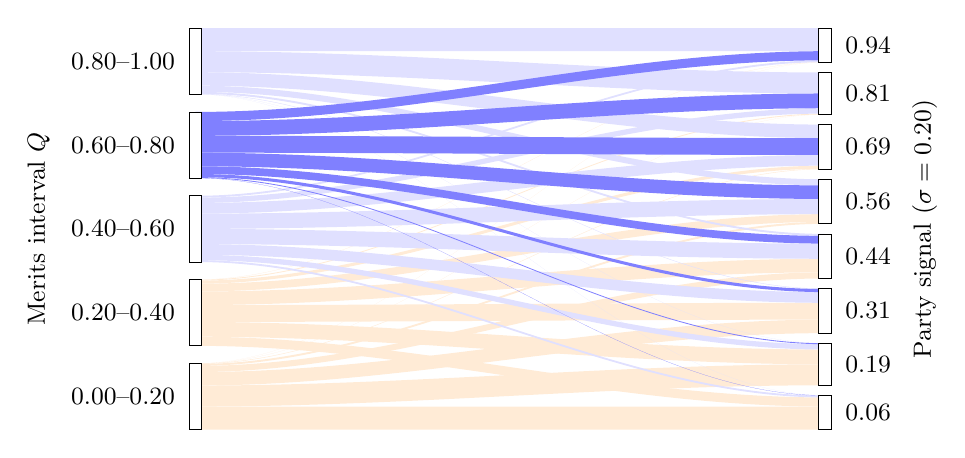
\begin{tikzpicture}[x=1cm,y=1cm,font=\small]\path[fill=orange!16!white,draw=none] (3.3,-5.1) .. controls (6,-5.1) and (8.6,-5.1) .. (11.3,-5.1) -- (11.3,-4.806673) .. controls (8.6,-4.806673) and (6,-4.806673) .. (3.3,-4.806673) -- cycle;
\path[fill=orange!16!white,draw=none] (3.3,-4.806673) .. controls (6,-4.806673) and (8.6,-4.536357) .. (11.3,-4.536357) -- (11.3,-4.269653) .. controls (8.6,-4.269653) and (6,-4.539969) .. (3.3,-4.539969) -- cycle;
\path[fill=orange!16!white,draw=none] (3.3,-4.539969) .. controls (6,-4.539969) and (8.6,-3.874105) .. (11.3,-3.874105) -- (11.3,-3.702913) .. controls (8.6,-3.702913) and (6,-4.368778) .. (3.3,-4.368778) -- cycle;
\path[fill=orange!16!white,draw=none] (3.3,-4.368778) .. controls (6,-4.368778) and (8.6,-3.179626) .. (11.3,-3.179626) -- (11.3,-3.102094) .. controls (8.6,-3.102094) and (6,-4.291246) .. (3.3,-4.291246) -- cycle;
\path[fill=orange!16!white,draw=none] (3.3,-4.291246) .. controls (6,-4.291246) and (8.6,-2.485714) .. (11.3,-2.485714) -- (11.3,-2.460979) .. controls (8.6,-2.460979) and (6,-4.266511) .. (3.3,-4.266511) -- cycle;
\path[fill=orange!16!white,draw=none] (3.3,-4.266511) .. controls (6,-4.266511) and (8.6,-1.791803) .. (11.3,-1.791803) -- (11.3,-1.786258) .. controls (8.6,-1.786258) and (6,-4.260966) .. (3.3,-4.260966) -- cycle;
\path[fill=orange!16!white,draw=none] (3.3,-4.260966) .. controls (6,-4.260966) and (8.6,-1.097324) .. (11.3,-1.097324) -- (11.3,-1.096453) .. controls (8.6,-1.096453) and (6,-4.260095) .. (3.3,-4.260095) -- cycle;
\path[fill=orange!16!white,draw=none] (3.3,-4.260095) .. controls (6,-4.260095) and (8.6,-0.435071) .. (11.3,-0.435071) -- (11.3,-0.434976) .. controls (8.6,-0.434976) and (6,-4.26) .. (3.3,-4.26) -- cycle;
\path[fill=orange!16!white,draw=none] (3.3,-4.035) .. controls (6,-4.035) and (8.6,-4.806673) .. (11.3,-4.806673) -- (11.3,-4.690854) .. controls (8.6,-4.690854) and (6,-3.919181) .. (3.3,-3.919181) -- cycle;
\path[fill=orange!16!white,draw=none] (3.3,-3.919181) .. controls (6,-3.919181) and (8.6,-4.269653) .. (11.3,-4.269653) -- (11.3,-4.082208) .. controls (8.6,-4.082208) and (6,-3.731736) .. (3.3,-3.731736) -- cycle;
\path[fill=orange!16!white,draw=none] (3.3,-3.731736) .. controls (6,-3.731736) and (8.6,-3.702913) .. (11.3,-3.702913) -- (11.3,-3.48895) .. controls (8.6,-3.48895) and (6,-3.517773) .. (3.3,-3.517773) -- cycle;
\path[fill=orange!16!white,draw=none] (3.3,-3.517773) .. controls (6,-3.517773) and (8.6,-3.102094) .. (11.3,-3.102094) -- (11.3,-2.929718) .. controls (8.6,-2.929718) and (6,-3.345397) .. (3.3,-3.345397) -- cycle;
\path[fill=orange!16!white,draw=none] (3.3,-3.345397) .. controls (6,-3.345397) and (8.6,-2.460979) .. (11.3,-2.460979) -- (11.3,-2.36301) .. controls (8.6,-2.36301) and (6,-3.247428) .. (3.3,-3.247428) -- cycle;
\path[fill=orange!16!white,draw=none] (3.3,-3.247428) .. controls (6,-3.247428) and (8.6,-1.786258) .. (11.3,-1.786258) -- (11.3,-1.747038) .. controls (8.6,-1.747038) and (6,-3.208208) .. (3.3,-3.208208) -- cycle;
\path[fill=orange!16!white,draw=none] (3.3,-3.208208) .. controls (6,-3.208208) and (8.6,-1.096453) .. (11.3,-1.096453) -- (11.3,-1.08542) .. controls (8.6,-1.08542) and (6,-3.197174) .. (3.3,-3.197174) -- cycle;
\path[fill=orange!16!white,draw=none] (3.3,-3.197174) .. controls (6,-3.197174) and (8.6,-0.434976) .. (11.3,-0.434976) -- (11.3,-0.432802) .. controls (8.6,-0.432802) and (6,-3.195) .. (3.3,-3.195) -- cycle;
\path[fill=blue!12!white,draw=none] (3.3,-2.97) .. controls (6,-2.97) and (8.6,-4.690854) .. (11.3,-4.690854) -- (11.3,-4.667198) .. controls (8.6,-4.667198) and (6,-2.946345) .. (3.3,-2.946345) -- cycle;
\path[fill=blue!12!white,draw=none] (3.3,-2.946345) .. controls (6,-2.946345) and (8.6,-4.082208) .. (11.3,-4.082208) -- (11.3,-4.01458) .. controls (8.6,-4.01458) and (6,-2.878716) .. (3.3,-2.878716) -- cycle;
\path[fill=blue!12!white,draw=none] (3.3,-2.878716) .. controls (6,-2.878716) and (8.6,-3.48895) .. (11.3,-3.48895) -- (11.3,-3.352962) .. controls (8.6,-3.352962) and (6,-2.742728) .. (3.3,-2.742728) -- cycle;
\path[fill=blue!12!white,draw=none] (3.3,-2.742728) .. controls (6,-2.742728) and (8.6,-2.929718) .. (11.3,-2.929718) -- (11.3,-2.73699) .. controls (8.6,-2.73699) and (6,-2.55) .. (3.3,-2.55) -- cycle;
\path[fill=blue!12!white,draw=none] (3.3,-2.55) .. controls (6,-2.55) and (8.6,-2.36301) .. (11.3,-2.36301) -- (11.3,-2.170282) .. controls (8.6,-2.170282) and (6,-2.357272) .. (3.3,-2.357272) -- cycle;
\path[fill=blue!12!white,draw=none] (3.3,-2.357272) .. controls (6,-2.357272) and (8.6,-1.747038) .. (11.3,-1.747038) -- (11.3,-1.61105) .. controls (8.6,-1.61105) and (6,-2.221284) .. (3.3,-2.221284) -- cycle;
\path[fill=blue!12!white,draw=none] (3.3,-2.221284) .. controls (6,-2.221284) and (8.6,-1.08542) .. (11.3,-1.08542) -- (11.3,-1.017792) .. controls (8.6,-1.017792) and (6,-2.153655) .. (3.3,-2.153655) -- cycle;
\path[fill=blue!12!white,draw=none] (3.3,-2.153655) .. controls (6,-2.153655) and (8.6,-0.432802) .. (11.3,-0.432802) -- (11.3,-0.409146) .. controls (8.6,-0.409146) and (6,-2.13) .. (3.3,-2.13) -- cycle;
\path[fill=blue!12!white,draw=none] (3.3,-0.84) .. controls (6,-0.84) and (8.6,-4.665024) .. (11.3,-4.665024) -- (11.3,-4.664929) .. controls (8.6,-4.664929) and (6,-0.839905) .. (3.3,-0.839905) -- cycle;
\path[fill=blue!12!white,draw=none] (3.3,-0.839905) .. controls (6,-0.839905) and (8.6,-4.003547) .. (11.3,-4.003547) -- (11.3,-4.002676) .. controls (8.6,-4.002676) and (6,-0.839034) .. (3.3,-0.839034) -- cycle;
\path[fill=blue!12!white,draw=none] (3.3,-0.839034) .. controls (6,-0.839034) and (8.6,-3.313742) .. (11.3,-3.313742) -- (11.3,-3.308197) .. controls (8.6,-3.308197) and (6,-0.833489) .. (3.3,-0.833489) -- cycle;
\path[fill=blue!12!white,draw=none] (3.3,-0.833489) .. controls (6,-0.833489) and (8.6,-2.639021) .. (11.3,-2.639021) -- (11.3,-2.614286) .. controls (8.6,-2.614286) and (6,-0.808754) .. (3.3,-0.808754) -- cycle;
\path[fill=blue!12!white,draw=none] (3.3,-0.808754) .. controls (6,-0.808754) and (8.6,-1.997906) .. (11.3,-1.997906) -- (11.3,-1.920374) .. controls (8.6,-1.920374) and (6,-0.731222) .. (3.3,-0.731222) -- cycle;
\path[fill=blue!12!white,draw=none] (3.3,-0.731222) .. controls (6,-0.731222) and (8.6,-1.397087) .. (11.3,-1.397087) -- (11.3,-1.225895) .. controls (8.6,-1.225895) and (6,-0.560031) .. (3.3,-0.560031) -- cycle;
\path[fill=blue!12!white,draw=none] (3.3,-0.560031) .. controls (6,-0.560031) and (8.6,-0.830347) .. (11.3,-0.830347) -- (11.3,-0.563643) .. controls (8.6,-0.563643) and (6,-0.293327) .. (3.3,-0.293327) -- cycle;
\path[fill=blue!12!white,draw=none] (3.3,-0.293327) .. controls (6,-0.293327) and (8.6,-0.293327) .. (11.3,-0.293327) -- (11.3,0) .. controls (8.6,0) and (6,0) .. (3.3,0) -- cycle;
\path[fill=blue!50!white,draw=none] (3.3,-1.905) .. controls (6,-1.905) and (8.6,-4.667198) .. (11.3,-4.667198) -- (11.3,-4.665024) .. controls (8.6,-4.665024) and (6,-1.902826) .. (3.3,-1.902826) -- cycle;
\path[fill=blue!50!white,draw=none] (3.3,-1.902826) .. controls (6,-1.902826) and (8.6,-4.01458) .. (11.3,-4.01458) -- (11.3,-4.003547) .. controls (8.6,-4.003547) and (6,-1.891792) .. (3.3,-1.891792) -- cycle;
\path[fill=blue!50!white,draw=none] (3.3,-1.891792) .. controls (6,-1.891792) and (8.6,-3.352962) .. (11.3,-3.352962) -- (11.3,-3.313742) .. controls (8.6,-3.313742) and (6,-1.852572) .. (3.3,-1.852572) -- cycle;
\path[fill=blue!50!white,draw=none] (3.3,-1.852572) .. controls (6,-1.852572) and (8.6,-2.73699) .. (11.3,-2.73699) -- (11.3,-2.639021) .. controls (8.6,-2.639021) and (6,-1.754603) .. (3.3,-1.754603) -- cycle;
\path[fill=blue!50!white,draw=none] (3.3,-1.754603) .. controls (6,-1.754603) and (8.6,-2.170282) .. (11.3,-2.170282) -- (11.3,-1.997906) .. controls (8.6,-1.997906) and (6,-1.582227) .. (3.3,-1.582227) -- cycle;
\path[fill=blue!50!white,draw=none] (3.3,-1.582227) .. controls (6,-1.582227) and (8.6,-1.61105) .. (11.3,-1.61105) -- (11.3,-1.397087) .. controls (8.6,-1.397087) and (6,-1.368264) .. (3.3,-1.368264) -- cycle;
\path[fill=blue!50!white,draw=none] (3.3,-1.368264) .. controls (6,-1.368264) and (8.6,-1.017792) .. (11.3,-1.017792) -- (11.3,-0.830347) .. controls (8.6,-0.830347) and (6,-1.180819) .. (3.3,-1.180819) -- cycle;
\path[fill=blue!50!white,draw=none] (3.3,-1.180819) .. controls (6,-1.180819) and (8.6,-0.409146) .. (11.3,-0.409146) -- (11.3,-0.293327) .. controls (8.6,-0.293327) and (6,-1.065) .. (3.3,-1.065) -- cycle;
\coordinate (axis-midline-0) at (0,-2.55);
\path[fill=white,draw=black,line width=0.3pt] (3.22,-5.1) rectangle (3.38,-4.26);
\node[anchor=east,fill=white,inner sep=2pt] (bucket-0-0-0) at (3.12,-4.68) {0.00--0.20};
\path[fill=white,draw=black,line width=0.3pt] (3.22,-4.035) rectangle (3.38,-3.195);
\node[anchor=east,fill=white,inner sep=2pt] (bucket-0-0-1) at (3.12,-3.615) {0.20--0.40};
\path[fill=white,draw=black,line width=0.3pt] (3.22,-2.97) rectangle (3.38,-2.13);
\node[anchor=east,fill=white,inner sep=2pt] (bucket-0-0-2) at (3.12,-2.55) {0.40--0.60};
\path[fill=white,draw=black,line width=0.3pt] (3.22,-1.905) rectangle (3.38,-1.065);
\node[anchor=east,fill=white,inner sep=2pt] (bucket-0-0-3) at (3.12,-1.485) {0.60--0.80};
\path[fill=white,draw=black,line width=0.3pt] (3.22,-0.84) rectangle (3.38,0);
\node[anchor=east,fill=white,inner sep=2pt] (bucket-0-0-4) at (3.12,-0.42) {0.80--1.00};
\node[fit=(bucket-0-0-0) (bucket-0-0-1) (bucket-0-0-2) (bucket-0-0-3) (bucket-0-0-4),inner sep=0pt] (source-labels-0) {};
\coordinate (axis-title-0-0) at (source-labels-0.west |- axis-midline-0);
\node[rotate=90,anchor=south,inner sep=0pt] at ([xshift=-0.18cm]axis-title-0-0) {Merits interval $Q$};
\path[fill=white,draw=black,line width=0.3pt] (11.22,-5.1) rectangle (11.38,-4.664929);
\node[anchor=west,fill=white,inner sep=2pt] (bucket-0-1-0) at (11.48,-4.882464) {0.06};
\path[fill=white,draw=black,line width=0.3pt] (11.22,-4.536357) rectangle (11.38,-4.002676);
\node[anchor=west,fill=white,inner sep=2pt] (bucket-0-1-1) at (11.48,-4.269517) {0.19};
\path[fill=white,draw=black,line width=0.3pt] (11.22,-3.874105) rectangle (11.38,-3.308197);
\node[anchor=west,fill=white,inner sep=2pt] (bucket-0-1-2) at (11.48,-3.591151) {0.31};
\path[fill=white,draw=black,line width=0.3pt] (11.22,-3.179626) rectangle (11.38,-2.614286);
\node[anchor=west,fill=white,inner sep=2pt] (bucket-0-1-3) at (11.48,-2.896956) {0.44};
\path[fill=white,draw=black,line width=0.3pt] (11.22,-2.485714) rectangle (11.38,-1.920374);
\node[anchor=west,fill=white,inner sep=2pt] (bucket-0-1-4) at (11.48,-2.203044) {0.56};
\path[fill=white,draw=black,line width=0.3pt] (11.22,-1.791803) rectangle (11.38,-1.225895);
\node[anchor=west,fill=white,inner sep=2pt] (bucket-0-1-5) at (11.48,-1.508849) {0.69};
\path[fill=white,draw=black,line width=0.3pt] (11.22,-1.097324) rectangle (11.38,-0.563643);
\node[anchor=west,fill=white,inner sep=2pt] (bucket-0-1-6) at (11.48,-0.830483) {0.81};
\path[fill=white,draw=black,line width=0.3pt] (11.22,-0.435071) rectangle (11.38,0);
\node[anchor=west,fill=white,inner sep=2pt] (bucket-0-1-7) at (11.48,-0.217536) {0.94};
\node[fit=(bucket-0-1-0) (bucket-0-1-1) (bucket-0-1-2) (bucket-0-1-3) (bucket-0-1-4) (bucket-0-1-5) (bucket-0-1-6) (bucket-0-1-7),inner sep=0pt] (destination-labels-0) {};
\coordinate (axis-title-0-1) at (destination-labels-0.east |- axis-midline-0);
\node[rotate=90,anchor=north,inner sep=0pt] at ([xshift=0.18cm]axis-title-0-1) {Party signal ($\sigma=0.20$)};
\end{tikzpicture}
\end{document}

